\documentclass{article}

\usepackage{fullpage}
\usepackage{color}
\usepackage{amsmath}
\usepackage{url}
\usepackage{verbatim}
\usepackage{graphicx}
\usepackage{parskip}
\usepackage{amssymb}
\usepackage{nicefrac}
\usepackage{listings}


% Colors
\definecolor{blu}{rgb}{0,0,1}
\def\blu#1{{\color{blu}#1}}
\definecolor{gre}{rgb}{0,.5,0}
\def\gre#1{{\color{gre}#1}}
\definecolor{red}{rgb}{1,0,0}
\def\red#1{{\color{red}#1}}
\def\norm#1{\|#1\|}

% Math
\def\R{\mathbb{R}}
\def\argmax{\mathop{\rm arg\,max}}
\def\argmin{\mathop{\rm arg\,min}}
\newcommand{\mat}[1]{\begin{bmatrix}#1\end{bmatrix}}
\newcommand{\alignStar}[1]{\begin{align*}#1\end{align*}}
\def\half{\frac 1 2}

% LaTeX
\newcommand{\fig}[2]{\includegraphics[width=#1\textwidth]{#2}}
\newcommand{\centerfig}[2]{\begin{center}\includegraphics[width=#1\textwidth]{#2}\end{center}}
\newcommand{\matCode}[1]{\lstinputlisting[language=Matlab]{a2f/#1.m}}
\def\items#1{\begin{itemize}#1\end{itemize}}
\def\enum#1{\begin{enumerate}#1\end{enumerate}}

\def\rubric#1{\gre{Rubric: \{#1\}}}{}

\begin{document}

\title{CPSC 340 Assignment 2 (due Friday January 26th at 9:00pm)}
\author{}
\date{}
\maketitle
\vspace{-4em}

\section*{Instructions}
\rubric{mechanics:5}

The above points are allocated for compliance with the CPSC 340 homework submission instructions:\\
\url{https://github.ugrad.cs.ubc.ca/CPSC340-2017W-T2/home/blob/master/homework_instructions.md}

\blu{NOTE: for this assignment you'll need to separately download the data from the home repo.
It can't be delivered in the normal way due to a limitation of the way we're using GitHub.}

\section{Naive Bayes}

In this section we'll implement naive Bayes, a very fast classification method that is often surprisingly accurate for text data with simple representations like bag of words.



\subsection{Naive Bayes by Hand}
\rubric{reasoning:3}

Consider the dataset below, which has $10$ training examples and $2$ features:
\[
X = \begin{bmatrix}0 & 1\\1 & 1\\ 0 & 0\\ 1 & 1\\ 1 & 1\\ 0 & 0\\  1 & 0\\  1 & 0\\  1 & 1\\  1 &0\end{bmatrix}, \quad y = \begin{bmatrix}1\\1\\1\\1\\1\\1\\0\\0\\0\\0\end{bmatrix}.
\]
Suppose you believe that a naive Bayes model would be appropriate for this dataset, and you want to classify the following test example:
\[
\hat{x} = \begin{bmatrix}1 & 0\end{bmatrix}.
\]

\blu{(a) Compute the estimates of the class prior probabilities} (you don't need to show any work):
\items{
\item$ p(y = 1)$.
 \textcolor{gre}{\\Answer: 6/10}
\item $p(y = 0)$.
 \textcolor{gre}{\\Answer: 4/10}
}

\blu{(b) Compute the estimates of the 4 conditional probabilities required by naive Bayes for this example}  (you don't need to show any work):
\items{
\item $p(x_1 = 1 | y = 1)$.
 \textcolor{gre}{\\Answer: 1/2}
\item $p(x_2 = 0 | y = 1)$.
 \textcolor{gre}{\\Answer: 1/3}
\item $p(x_1 = 1 | y = 0)$.
 \textcolor{gre}{\\Answer: 1}
\item $p(x_2 = 0 | y = 0)$.
 \textcolor{gre}{\\Answer: 3/4}
}

\blu{(c) Under the naive Bayes model and your estimates of the above probabilities, what is the most likely label for the test example? (Show your work.)}
\newline
\gre{Answer: The probability that the label for test example is 1 is: \newline $p(y=1|x1=1,x2=0)$ = $p(x1=1|y=1)$*$p(x2=0|y=1)$*$p(y=1)$ = 1/2 * 1/3 * 3/5 = 1/10.
\newline \newline The probability that the label for test example is 0 is: \newline $p(y=0 | x1=1,x2=0)$ = $p(x1=1|y=0)$*$p(x2=0|y=0)$*$p(y=0)$ = 1 * 3/4 * 2/5 = 3/10.
\newline \newline Therefore, the most likely label 0.}

\subsection{Bag of Words}
\rubric{reasoning:3}

If you run \texttt{python main.py -q 1.2}, it will load the following dataset:
\enum{
\item $X$: A sparse binary matrix. Each row corresponds to a newsgroup post, and each column corresponds to whether a particular word was used in the post. A value of $1$ means that the word occured in the post.
\item $wordlist$: The set of words that correspond to each column.
\item $y$: A vector with values $1$ through $4$, with the value corresponding to the newsgroup that the post came from.
\item $groupnames$: The names of the four newsgroups.
\item $Xvalidate$ and $yvalidate$: the word lists and newsgroup labels for additional newsgroup posts.
}
\blu{Answer the following}:
\enum{
\item Which word corresponds to column 50 of $X$?
 \textcolor{gre}{\\Answer: Lunar}
\item Which words are present in training example 500?
 \textcolor{gre}{\\Answer: car, fact, gun, video}
\item Which newsgroup name does training example 500 come from?
 \textcolor{gre}{\\Answer: talk.*}
}

\subsection{Naive Bayes Implementation}
\rubric{code:5}

If you run \texttt{python main.py -q 1.3}
it will load the newsgroups dataset and report the test error for a random forest,
and also fit the basic naive Bayes model and report the test error.

The \texttt{predict()} function of the naive Bayes classifier is already implemented.
However, in \texttt{fit()}
the calculation of the variable \texttt{p\_xy} is incorrect
(right now, it just sets all values to $1/2$).
\blu{Modify this function so that \texttt{p\_xy} correctly
computes the conditional probabilities of these values based on the
frequencies in the data set. Hand in your code and the validation error that you obtain.
Also, briefly comment on the accuracy as compared to the random forest and scikit-learn's naive Bayes implementation.}

\gre{Answer: URL for naive\_bayes.py code: \url{https://github.ugrad.cs.ubc.ca/CPSC340-2017W-T2/g5e0b_u7p1b_a2/blob/master/code/naive_bayes.py}.} \newline
\gre{Answer: The validation error obtained is 0.188. This validation error was better than Random Forest (sklearn's) validation error, which was 0.198. This validation error was slightly worse than sklearn's Naive Bayes validation error, which was 0.187}

\subsection{Laplace smoothing}
\rubric{code:1}

\blu{Do the following:}
\enum{
\item Modify your code so that it uses Laplace smoothing, with $\beta$
as a parameter taken in by the constructor.
\newline
\gre{Answer: Link to naive\_bayes.py: \url{https://github.ugrad.cs.ubc.ca/CPSC340-2017W-T2/g5e0b_u7p1b_a2/blob/master/code/naive_bayes.py}.}
\item Did you need to modify your fit function, predict function, or both?
\newline
\gre{Answer: We only needed to modify the fit function}
\item Take a look at the documentation for the scikit-learn version of naive Bayes the code is using. How much Laplace smoothing does it use by default? Using the same amount of smoothing with your code, do you get the same results?
\newline
\gre{Answer: The scikit-learn version of naive Bayes uses a smoothing value of 1 by default. Using the same amount of smoothing with our code, we obtained a validation error of 0.188 while scikit-learn's version obtained a validation error of 0.187}
}

\subsection{Runtime of Naive Bayes for Discrete Data}
\rubric{reasoning:3}

Assume you have the following setup:
\items{
\item The training set has $n$ objects each with $d$ features.
\item The test set has $t$ objects with $d$ features.
\item Each feature can have up to $c$ discrete values (you can assume $c \leq n$).
\item There are $k$ class labels (you can assume $k \leq n$)
}
You can implement the training phase of a naive Bayes classifier in this setup in $O(nd)$, since you only need to do a constant amount of work for each $X(i,j)$ value. (You do not have to actually implement it in this way for the previous question, but you should think about how this could be done). \blu{What is the cost of classifying $t$ test examples with the model?}
\newline
\gre{Answer: The cost of classifying t test examples with the model is O(TDK)}



\section{Random Forests}

\subsection{Implementation}
\rubric{reasoning:7}

The file \emph{vowels.pkl} contains a supervised learning dataset where we are trying to predict which of the 11 ``steady-state'' English vowels that a speaker is trying to pronounce.

You are provided with a \texttt{RandomStump} class that differs from
\texttt{DecisionStump} in two ways: it uses the information gain splitting criterion
(instead of classification accuracy), and
it only considers $\lfloor \sqrt{d} \rfloor$ randomly-chosen features.\footnote{The notation $\lfloor x\rfloor$ means the ``floor'' of $x$, or ``$x$ rounded down''. You can compute this with \texttt{np.floor(x)} or \texttt{math.floor(x)}.}
You are also provided with a \texttt{RandomTree} class that is exactly the same as
\texttt{DecisionTree} except that it uses \texttt{RandomStump} instead of
\texttt{DecisionStump} and it takes a bootstrap sample of the data before fitting.
In other words, \texttt{RandomTree} is the entity we discussed in class, which
makes up a random forest.

If you run \texttt{python main.py -q 2} it will fit a deep \texttt{DecisionTree}
using the information gain splitting criterion. You will notice that the model overfits badly.


\blu{
\enum{
\item Why doesn't the random tree model have a training error of 0?
\newline
\gre{Answer: The random tree model doesn't have a training error of 0 since only approximately 63\% of the training data is present in the bootstrap sample. Therefore, not all label predictions based on the training data will be correct, resulting in a training error $>$ 0}
\item Create a class \texttt{RandomForest} in a file called \texttt{random\string_forest.py} that takes in hyperparameters \texttt{num\string_trees} and \texttt{max\string_depth} and
fits \texttt{num\string_trees} random trees each with maximum depth \texttt{max\string_depth}. For prediction, have all trees predict and then take the mode, allowing errors to be minimized.
\newline
\gre{Answer: Link to RandomForest: \url{https://github.ugrad.cs.ubc.ca/CPSC340-2017W-T2/g5e0b_u7p1b_a2/blob/master/code/random_forest.py}.}
\item Using 50 trees, and a max depth of $\infty$, report the training and testing error. Compare this to what we got with a single \texttt{DecisionTree} and with a single \texttt{RandomTree}. Are the results what you expected? Discuss.
\newline
\gre{Answer: Using 50 trees and a max depth of infinity we got a training error of 0 and a test error of 0.174. Using a single DecisionTree we got a training error of 0 and a testing error of 0.367. Using a single RandomTree we got a training error of 0.117 and a testing error of 0.481. The results met with our expectations. The RandomTree generated a positive training error since not all of the training data were present in the bootstrap sample. The RandomTree generated the highest test error, followed by the DecisionTree, and then the RandomForest. These results were expected since the RandomTree utilized the least training data, and thus is likely to be the most biased. RandomForest had the lowest test error, which is expected since it reduces overfitting.}
\item Compare your implementation with scikit-learn's \texttt{RandomForestClassifier} for both speed and accuracy, and briefly discuss. You can use all default hyperparameters if you wish, or you can try changing them.
\newline
\gre{Answer: Our implementation of RandomForest took 21 seconds to execute for 50 trees with an infinite max depth while scikit-learn’s RandomForestClassifier took 0.16 seconds to execute for the same hyperparameters. The test error for our implementation was 0.189 while the test error for scikit-learn’s implementation was 0.155. The training errors for both implementations were 0. Overall, scikit-learn’s implementation was faster and had a smaller test error.}
}
}

\subsection{Very-Short Answer Questions}
\rubric{reasoning:3}

\blu{\enum{
\item What is a a disadvantage of using a very-large number of trees in a random forest classifier?
\newline
\gre{Answer: A disadvantage of using a very-large number of trees is the runtime will be very slow}
\item Your random forest classifier has a training error of 0 and a very high test error. Which ones of the following could help performance?
\enum{
\item Increase the maximum depth of the trees in your forest.
\item Decrease the maximum depth of the trees in your forest.
\item Increase the amout of data you consider for each tree (Collect more data and use $2n$ objects instead of $n$).
\item Decrease the amount of data you consider for each tree (Use $0.8n$ objects instead of $n$).
\item Increase the number of features you consider for each tree.
\item Decrease the number of features you consider for each tree.
}
\gre{Answer: In order to help performance, one could: (B) decrease the maximum depth of the trees in your forest, (C) Increase the amount of data you consider for each tree (Collect more data and use $2n$ objects instead of $n$), and (E) decrease the number of features you consider for each tree}
\item Suppose that you were training on raw audio segments and trying to recognize vowel sounds. What could you do to encourage the final classifier to be invariant to translation?
\newline
\gre{Answer: In order to encourage the final classifier to be invariant to translation one could add transformed data (ex: sound clips consisting of vowel sounds starting after different times (speaking after 0 seconds, 0.1 second, 0.2 seconds of starting the audio clip, etc)) during training}
}
}

\section{Clustering}

If you run \verb|python main.py -q 3|, it will load a dataset with two features
and a very obvious clustering structure. It will then apply the $k$-means algorithm
with a random initialization. The result of applying the
algorithm will thus depend on the randomization, but a typical run might look like this:
\begin{figure}[h!]
\centerfig{.5}{../figs/kmeans_basic.png}
\caption{clustering figure 1}
\end{figure}
(Note that the colours are arbitrary -- this is the label switching issue.)
But the `correct' clustering (that was used to make the data) is this:
\begin{figure}[h!]
\centerfig{.5}{../figs/kmeans_good.png}
\caption{clustering figure 2}
\end{figure}
\subsection{Selecting among $k$-means Initializations}
\rubric{reasoning:5}

If you run the demo several times, it will find different clusterings. To select among clusterings for a \emph{fixed} value of $k$, one strategy is to minimize the sum of squared distances between examples $x_i$ and their means $w_{y_i}$,
\[
f(w_1,w_2,\dots,w_k,y_1,y_2,\dots,y_n) = \sum_{i=1}^n \norm{x_i - w_{y_i}}_2^2 = \sum_{i=1}^n \sum_{j=1}^d (x_{ij} - w_{y_ij})^2.
\]
 where $y_i$ is the index of the closest mean to $x_i$. This is a natural criterion because the steps of $k$-means alternately optimize this objective function in terms of the $w_c$ and the $y_i$ values.

 \blu{\enum{
 \item In the \emph{kmeans.py} file, add a new function called \emph{error} that takes the same input as the \emph{predict} function but that returns the value of this above objective function. Hand in your code.
 \textcolor{gre}{\\Answer: the URL of the code is: \url{https://github.ugrad.cs.ubc.ca/CPSC340-2017W-T2/g5e0b_u7p1b_a2/blob/master/code/kmeans.py}}
 \item What trend do you observe if you print the value of \emph{error} after each iteration of the $k$-means algorithm?
 \textcolor{gre}{\\Answer: The error monotonically decreases.}
 \item Using \texttt{plot\_2dclustering}, output the clustering obtained by running $k$-means 50 times (with $k=4$) and taking the one with the lowest error.
 \textcolor{gre}{\\Answer: The minimal error is 3071.468053, and the corresponding clustering is shown below.\\}
 \begin{figure}[h!]
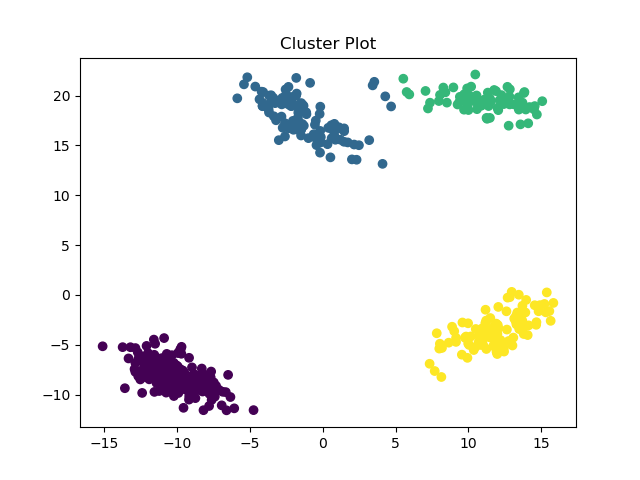
\includegraphics[width=0.8\textwidth]{C:/Users/wangzhen/Desktop/cpsc340/g5e0b_u7p1b_a2-master/figs/q3_1.png}
\caption{clustering figure 3.1}
\end{figure}
 \item Looking at the hyperparameters of scikit-learn's \texttt{KMeans}, explain the first four (\texttt{n\_clusters}, \texttt{init}, \texttt{n\_init}, \texttt{max\_iter}) very briefly.
 \textcolor{gre}{\\Answer: \texttt{n\_clusters} is the number of clusters to form as well as the number of centroids to generate. \texttt{init} is method for initialization including k-means++ and random. \texttt{n\_init} is number of time the k-means algorithm will be run with different centroid seeds. \texttt{max\_iter} is maximum number of iterations of the k-means algorithm for a single run.}
 }}


 \subsection{Selecting $k$ in $k$-means}
\rubric{reasoning:5}

 We now turn to the task of choosing the number of clusters $k$.

 \blu{\enum{
 \item Explain why the \emph{error} function should not be used to choose $k$.
 \textcolor{gre}{\\Answer: It is obvious that if we choose k equals to the number of examples, the error will be 0. Actually the error decreases with the increase of k, thus we only need to choose a larger k. This cannot be the reason to choose k.}
 \item Explain why even evaluating the \emph{error} function on test data still wouldn't be a suitable approach to choosing $k$.
 \textcolor{gre}{\\Answer: When k increases, it means the number of clusters increases. For the test data with new data, to get smaller error, choosing a larger k still works.}
 \item Hand in a plot of the minimum error found across 50 random initializations, as a function of $k$, taking $k$ from $1$ to $10$.
 \textcolor{gre}{\\Answer: The plot reflecting the relation between k and error is given below.\\}
  \begin{figure}[h!]
 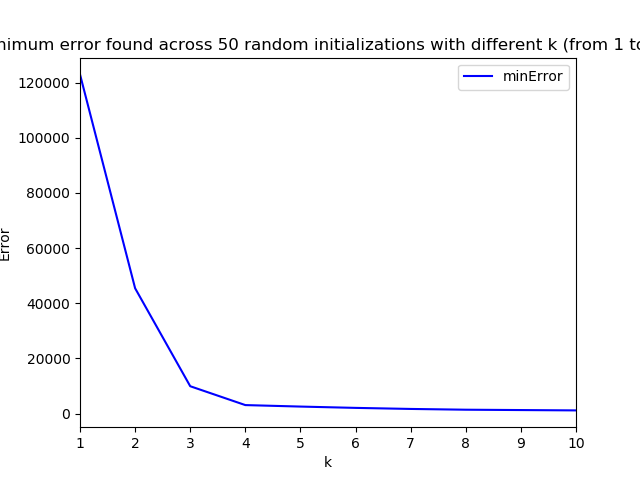
\includegraphics[width=0.8\textwidth]{C:/Users/wangzhen/Desktop/cpsc340/g5e0b_u7p1b_a2-master/figs/q3_2.png}
\caption{clustering figure 3.2}
\end{figure}
 \item The \emph{elbow method} for choosing $k$ consists of looking at the above plot and visually trying to choose the $k$ that makes the sharpest ``elbow" (the biggest change in slope). What values of $k$ might be reasonable according to this method? Note: there is not a single correct answer here; it is somewhat open to interpretation and there is a range of reasonable answers.
 \textcolor{gre}{\\Answer: As it is shown in the plot above, the reasonable k value should be 2, 3 or 4 with a big change in slope. }
 }}

 \subsection{$k$-medians}
\rubric{reasoning:5}

 The data in \emph{clusterData2.pkl} is the exact same as the above data, except it has 4 outliers that are very far away from the data.

 \blu{\enum{
 \item Using the \texttt{plot\_2dclustering} function, output the clustering obtained by running $k$-means 50 times (with $k=4$)  and taking the one with the lowest error. Are you satisfied with the result?
 \textcolor{gre}{\\Answer: The plot below shows the kmeans result for clusterData2.\\
  \begin{figure}[h!]
 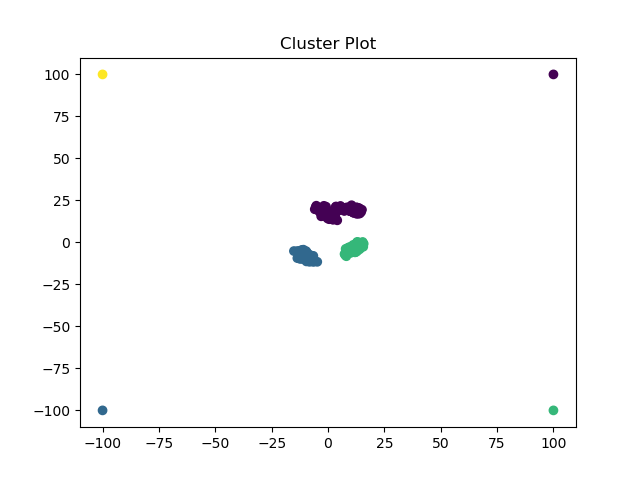
\includegraphics[width=0.8\textwidth]{C:/Users/wangzhen/Desktop/cpsc340/g5e0b_u7p1b_a2-master/figs/q3_3_kmeans.png}\\
\caption{clustering figure 3.3}
\end{figure}
 The min error is 59116.295803 which is too huge. I am not satisfied with the result.
 }
 \item What values of $k$ might be chosen by the elbow method for this dataset?
 \textcolor{gre}{\\Answer: The plot below shows the minimum error change with k increasing.\\
 \begin{figure}[h!]
 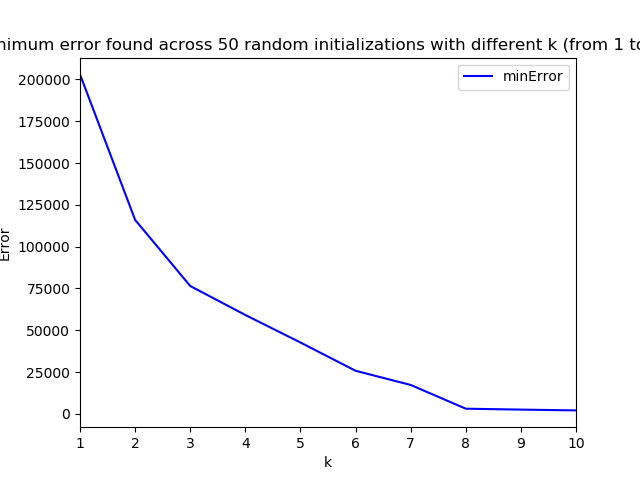
\includegraphics[width=0.8\textwidth]{C:/Users/wangzhen/Desktop/cpsc340/g5e0b_u7p1b_a2-master/figs/q3_3_kmeans_error.png}\\
\caption{clustering figure 3.3error}
\end{figure}
\\From this plot, we can find that the reasonable k is 2, 3 or 8. But when k=8, it does not make sense as there are 4 clusters only containing one point and the k=4 does not see a sharp elbow.}
 \item Implement the $k$-\emph{medians} algorithm, which assigns examples to the nearest $w_c$ in the L1-norm and to updates the $w_c$ by setting them to the ``median" of the points assigned to the cluster (we define the $d$-dimensional median as the concatenation of the median of the points along each dimension). Hand in your code and plot obtained with 50 random initializations for $k = 4$.
 \textcolor{gre}{\\Answer: The URL of the code is: \url{https://github.ugrad.cs.ubc.ca/CPSC340-2017W-T2/g5e0b_u7p1b_a2/blob/master/code/kmedians.py}. The plot of the result with k=4 is as below.\\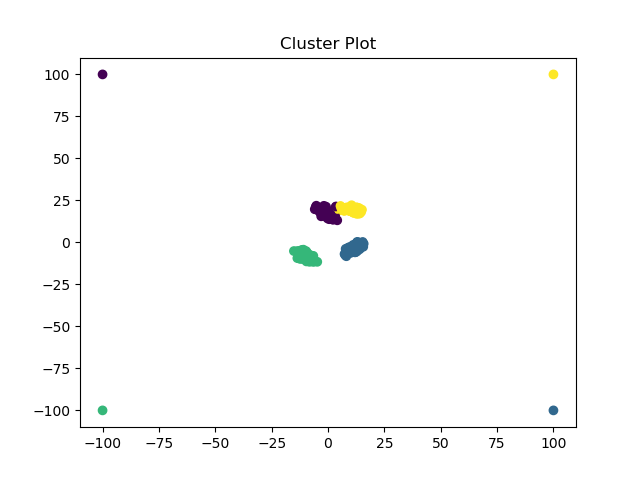
\includegraphics[width=0.8\textwidth]{C:/Users/wangzhen/Desktop/cpsc340/g5e0b_u7p1b_a2-master/figs/q3_3_kmedians.png}\\}
\item Using the L1-norm version of the error (where $y_i$ now represents the closest median in the L1-norm),
\[
f(w_1,w_2,\dots,w_k,y_1,y_2,\dots,y_n) = \sum_{i=1}^n \norm{x_i - w_{y_i}}_1 = \sum_{i=1}^n \sum_{j=1}^d |x_{ij} - w_{y_ij}|,
\]
what value of $k$ would be chosen by the elbow method under this strategy? Are you satisfied with this result?
\textcolor{gre}{\\Answer: The minimum error plot is shown as below.\\
 \begin{figure}[h!]
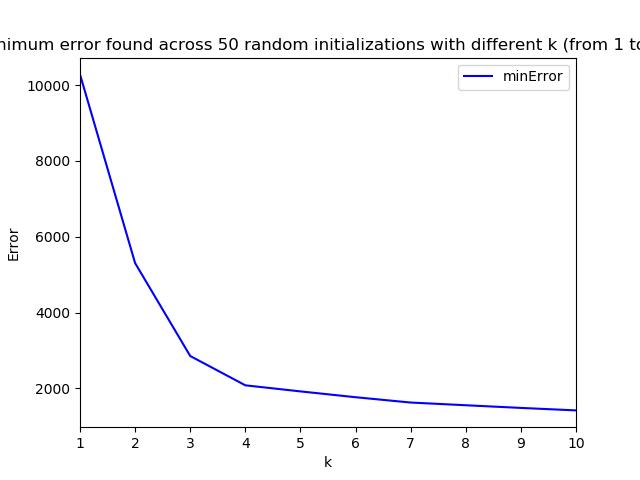
\includegraphics[width=0.8\textwidth]{C:/Users/wangzhen/Desktop/cpsc340/g5e0b_u7p1b_a2-master/figs/q3_3_kmedians_error.png}
\caption{clustering figure 3.3 kmedians error}
\end{figure}
\\The reasonable k is 2, 3 or 4. The error is much smaller than the kmeans thus I am satisfied with the result.}
}
}

\subsection{Density-Based Clustering}
\rubric{reasoning:2}

If you run \texttt{python main.py -q 3.4},
it will apply the basic density-based clustering algorithm to the dataset from the previous part.
The final output should look somewhat like this:\\
\fig{.49}{../figs/density}\fig{.49}{../figs/density2}\\
(The right plot is zoomed in to show the non-outlier part of the data.)
Even though we know that each object was generated from one of four clusters (and we have 4 outliers),
 the algorithm finds 6 clusters and does not assign some of the original non-outlier
  objects to any cluster. However, the clusters will change if we change the parameters
  of the algorithm. Find and report values for the two
  parameters, \texttt{eps} (which we called the ``radius'' in class) and \texttt{minPts},
   such that the density-based clustering method finds:
\blu{\enum{
\item The 4 ``true" clusters.
\item 3 clusters (merging the top two, which also seems like a reasonable interpretaition).
\item 2 clusters.
\item 1 cluster (consisting of the non-outlier points).
}
}
\textcolor{gre}{\\Answer: For clusterData2, we keep the minPts=3 and change eps.
\enum{
\item eps=3
\item eps=9
\item eps=15
\item eps=20
}}


\subsection{Very-Short Answer Questions}
\rubric{reasoning:3}

\blu{
\enum{
\item Does the standard $k$-means clustering algorithm always yield the optimal clustering solution for a given $k$?
\textcolor{gre}{\\Answer: No. For different initializations, it may not always converge to the optimal solution but a sub-optimal one. }
\item If your set out to minimize the distance between each point and its mean in a $k$-means clustering, what value of $k$ minimizes this cost? Is this value useful?
\textcolor{gre}{\\Answer: When k=n, the distance is minimized to 0. But it is not useful.}
\item Describe a dataset with $k$ clusters where $k$-means would not be able to find the true clusters.
\textcolor{gre}{\\Answer: Consider a condition with 2 clusters and there is a line between two points in one cluster going through the other cluster.}
\item Suppose that you had only two features and that they have very-different scales (like kilograms vs. milligrams). How would this affect the result of density-based clustering?
\textcolor{gre}{\\Answer: If the scales of features are really different, the expand of cluster may always add the one with smaller scale first as they will be much more possible to be in the neighbour cluster. This actually ignore the feature of smaller scale. Thus features should be of similar scales or should be normalized to similar scales. Actually, it is even difficult to choose proper minPts and eps in this condition.}
\item Name a key advantage and drawback of using a supervised outlier detection method rather than an unsupervised method?
\textcolor{gre}{\\Answer: For supervised outlier detection, if the outliers are similar to normal points, it can perform very well with high accuracy. However, if the outliers and the normal points are different, supervised method will not work and we have to use unsupervised method. }
}}



\section{Vector Quantization}
\rubric{reasoning:6}

Discovering object groups is one motivation for clustering. Another motivation is \emph{vector quantization}, where we find a prototype point for each cluster and replace points in the cluster by their prototype. If our inputs are images, vector quantization gives us a rudimentary image compression algorithm.

Your task is to implement image quantization in \emph{quantize\_image.py} with \texttt{quantize} and \texttt{dequantize} functions. The \texttt{quantize} function should take in an image and, using the pixels as examples and the 3 colour channels as features, run $k$-means clustering on the data with $2^b$ clusters for some hyperparameter $b$. The code should store the cluster means and return the cluster assignments. The \texttt{dequantize} function should return a version of the image (the same size as the original) where each pixel's orignal colour is replaced with the nearest prototype colour.

To understand why this is compression, consider the original image space. Say the image can take on the values $0,1,\ldots,254,255$ in each colour channel. Since $2^8=256$ this means we need 8 bits to represent each colour channel, for a total of 24 bits per pixel. Using our method, we are restricting each pixel to only take on one of $2^b$ colour values. In other words, we are compressing each pixel from a 24-bit colour representation to a $b$-bit colour representation by picking the $2^b$ prototype colours that are ``most representative'' given the content of the image. So, for example, if $b=6$ then we have 4x compression.

The loaded image contains a 3D-array representing the RGB values of a picture.
\blu{Implement the \emph{quantize} and \emph{dequantize} functions and show the image
obtained if you encode the colours using $1$, $2$, $4$, and $6$ bits with the provided image.}
You are welcome to use the provided implementation of $k$-means or the scikit-learn version.


\blu{\enum{
\item Hand in your \emph{quantizeImage} and \emph{deQuantizeImage} functions.
\item Show the image obtained if you encode the colours using $1$, $2$, $4$, and $6$ bits per pixel (instead of the original 24-bits).
\item Briefly comment on the prototype colours learned in case each, which are saved by the code.
}}
\textcolor{gre}{\\Answer:
\enum{
\item The URL of the code is: \url{https://github.ugrad.cs.ubc.ca/CPSC340-2017W-T2/g5e0b_u7p1b_a2/blob/master/code/quantize_image.py}.
\item The images obtained are shown below.\\
   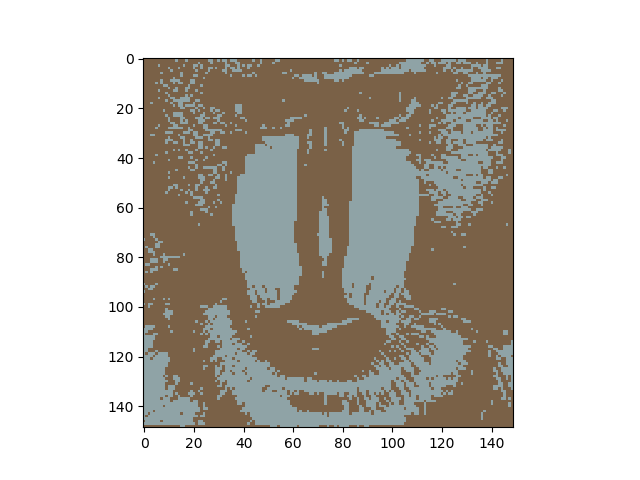
\includegraphics[width=0.8\textwidth]{C:/Users/wangzhen/Desktop/cpsc340/g5e0b_u7p1b_a2-master/figs/b_1_image.png}\\
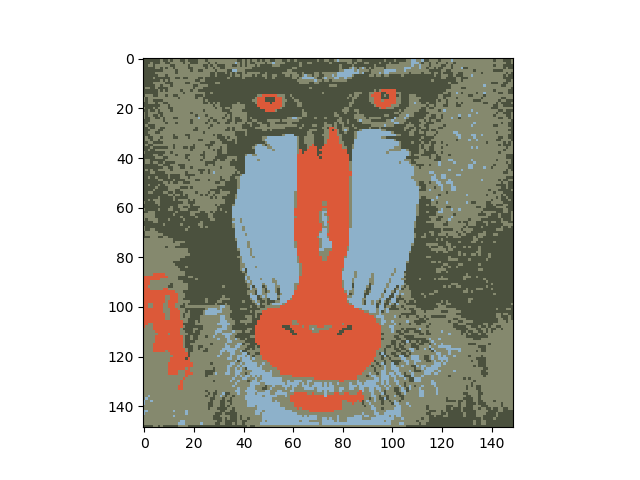
\includegraphics[width=0.8\textwidth]{C:/Users/wangzhen/Desktop/cpsc340/g5e0b_u7p1b_a2-master/figs/b_2_image.png}\\
    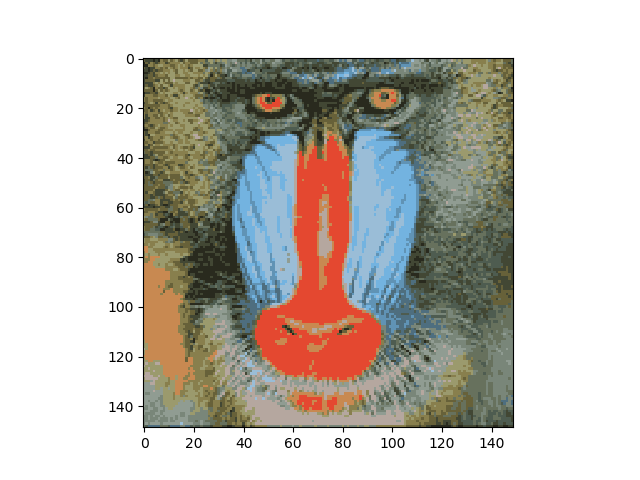
\includegraphics[width=0.8\textwidth]{C:/Users/wangzhen/Desktop/cpsc340/g5e0b_u7p1b_a2-master/figs/b_4_image.png}\\
    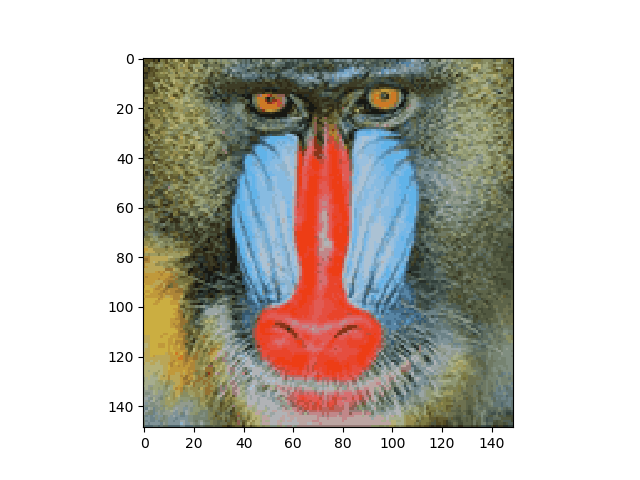
\includegraphics[width=0.8\textwidth]{C:/Users/wangzhen/Desktop/cpsc340/g5e0b_u7p1b_a2-master/figs/b_6_image.png}\\
\item The prototype of the colours are shown below.\\ 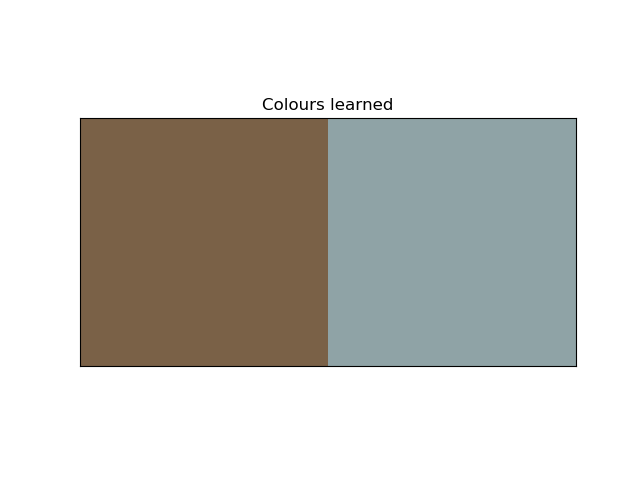
\includegraphics[width=0.8\textwidth]{C:/Users/wangzhen/Desktop/cpsc340/g5e0b_u7p1b_a2-master/figs/b_1_colours.png}\\
    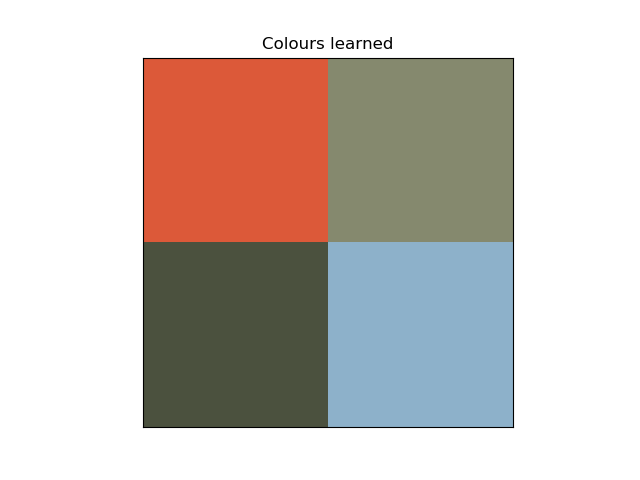
\includegraphics[width=0.8\textwidth]{C:/Users/wangzhen/Desktop/cpsc340/g5e0b_u7p1b_a2-master/figs/b_2_colours.png}\\
    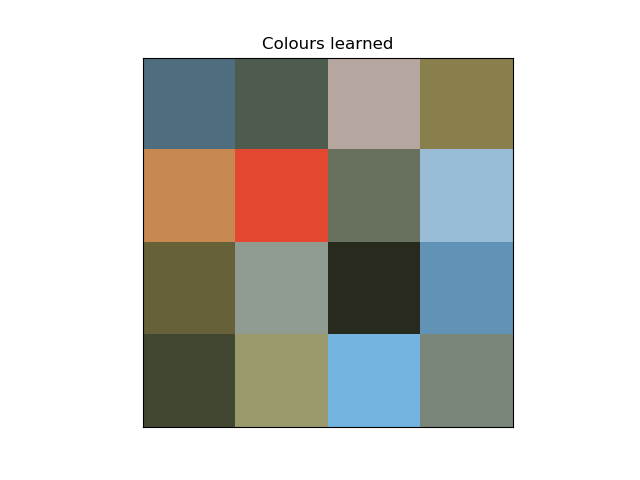
\includegraphics[width=0.8\textwidth]{C:/Users/wangzhen/Desktop/cpsc340/g5e0b_u7p1b_a2-master/figs/b_4_colours.png}\\
    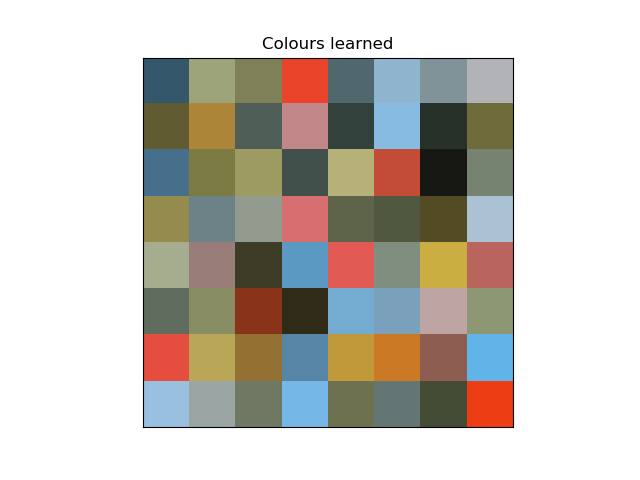
\includegraphics[width=0.8\textwidth]{C:/Users/wangzhen/Desktop/cpsc340/g5e0b_u7p1b_a2-master/figs/b_6_colours.png}\\
    From these figures, we can conclude that with b (or the number of clusters) increasing, the details of image are better displayed and the image looks smooth and more similar to the original image as more and more pixels are colored with better means and more kinds of colors are used as means. Based on the principle, it is obvious that the clusters of colors always in the region which could be the 'center' of this color considering its distribution of the whole image.
}}

\end{document}
